% FILE: sentiment.tex  Version 0.01
% AUTHOR: Uladzimir Sidarenka

% This is a modified version of the file main.tex developed by the
% University Duisburg-Essen, Duisburg, AG Prof. Dr. Günter Törner
% Verena Gondek, Andy Braune, Henning Kerstan Fachbereich Mathematik
% Lotharstr. 65., 47057 Duisburg entstanden im Rahmen des
% DFG-Projektes DissOnlineTutor in Zusammenarbeit mit der
% Humboldt-Universitaet zu Berlin AG Elektronisches Publizieren Joanna
% Rycko und der DNB - Deutsche Nationalbibliothek

\chapter{Sentiment Corpus}\label{chap:corpus}

A crucial prerequisite for proving any hypotheses in computational
linguistics is the existence of sufficiently big manually annotated
datasets, on which these conjectures could be tested.  Since there
were no human-labeled sentiment data for German Twitter that we were
aware of at the time of writing this chapter, we decided to create our
own corpus, which we will introduce in this part of the thesis.

We begin our introduction by describing the selection criteria and
tracking procedure that we used to collect the initial corpus data.
After presenting the annotation scheme, we perform an extensive
analysis of the inter-annotator agreement.  For this purpose, we
introduce two new versions of the popular $\kappa$ metric
\cite{Cohen:60}---binary and proportional kappa---which have been
specifically adjusted to the peculiarities of our annotation task.
Using these measures, we check the inter-coder reliability of
annotated sentiments, their targets and sources, polar terms and their
modifying elements (intensifiers, diminishers, and negations).  In the
final step, we estimate the correlation between the initial selection
rules and the number of labeled elements as well as the difficulty of
their annotation.

\section{Data Collection}

A common question that typically arises first when one starts creating
a new dataset is which selection criteria should be used in order to
collect the initial data.  Whereas for low-level NLP applications,
such as part-of-speech tagging or syntactic parsing, it typically
suffices to define the language domain to sample from (since the
phenomena of interest are usually frequent and uniformly spread), for
semantically demanding tasks, with many diverse ways of expression,
one also needs to consider various in-domain factors that might
significantly affect the final distribution, making the resulting
corpus either utterly sparse or excessively biased.

In order to minimize both of these risks (sparseness and bias), we
decided to use a compromise approach by gathering one part of the new
dataset from microblogs that were a priori more likely to have
sentiments (thus increasing the recall) and sampling the rest of the
corpus uniformly at random (thus reducing the bias).

As criteria that could help us get more opinions, we considered topic
and form of the tweets, assuming that some subjects, especially social
or political issues, would be more amenable to subjective statements.
Because we started creating the corpus in spring 2013, obvious choices
of opinion-rich topics to us were \emph{the papal conclave}, which
took place in March of that year, and \emph{the German federal
  elections}, which were held in autumn.  Since both of these events
implied some form of voting, we decided to counterbalance the election
specifics by including \emph{general political discussions} as the
third subject in our dataset.  Finally, to obey the second principle,
\ie{} to keep the corpus bias low, we sampled the rest of the data
from \emph{casual everyday conversations} without any prefiltering.

We collected messages for the first three groups by tracking German
microblogs between March and September 2013 through the public Twitter
API\footnote{\url{https://pypi.python.org/pypi/tweetstream}} with the
help of extensive keyword lists that described these topics.  For the
fourth category (casual everyday conversations), we used the complete
German Twitter snapshot \cite{Scheffler:14}, which includes
$\approx97\%$ of all German microblogs posted in April 2013.  This
way, we obtained a total of 27.4~M messages, with the snapshot corpus
being by far the most prolific source of the data.

%% For our work, the in-domain factors to consider were the topics and
%% the form of tweets.  Since we wanted our corpus to be as
%% representative as possible, we had to make sure that the topics we
%% choose for sampling lend themselves as fruitful opinion sources.  At
%% the same time, we did not want automatically generated ad and news
%% tweets to spoil our data and also introduced additional formal
%% criteria (described below) that the tweets had to satisfy in order to
%% be chosen.  But then again, applying these restriction might make the
%% dataset excessively biased, so we did allow for a certain proportion
%% of tweets being selected even if they did not conform to our
%% constraints.

%% Politics: 59,531 messages, keywords: Altmaier, Wowereit, Minister,
%% Bundeskanzleramt, Schwarz-Gelb

%% Papst: 51,579 messages, keywords: papst, pabst, konklave, Vatikan
%% General Tweets: 51,579 messages, keywords: papst, pabst, konklave, Vatikan

%% Federal Elections: 3,131,315 messages, keywords:

%% General: 24,179,871 messages, keywords:

In the next step, we divided all tweets of the same topic into three
groups based on the following formal criteria:
\begin{itemize}
\item We put all messages that contained at least one polar term from
  the sentiment lexicon of \citet{Remus:10} into the first group;
\item Microblogs that did not satisfy the first condition, but had at
  least one exclamation mark or emoticon were allocated to the second
  group;
\item All remaining microblogs were assigned to the third category.
\end{itemize}
A detailed breakdown of the resulting distribution across topics and
formal groups is given in Table~\ref{snt:tbl:corp:topic-bins}.
\begin{table}[hbt!]\small
  \begin{center}
    \bgroup \setlength\tabcolsep{0.13\tabcolsep}\scriptsize
    \begin{tabular}{l*{5}{>{\centering\arraybackslash}p{0.155\textwidth}}}
      \toprule
      & \multicolumn{4}{c}{\bfseries Formal Criterion} & \\\cmidrule{2-5}

      \multirow{-2}{0.2\columnwidth}{\centering\bfseries
      Topic} & Polar Terms & Emoticons & Remaining Tweets & Total &\multirow{-2}{0.12\textwidth}{\centering\bfseries Sample\\ Keywords}\\\midrule

      Federal Elections & 537,083 (22.38\%) & 50,567 (2.1\%) & 1,811,742 (75.5\%) & 2,399,392 & \tiny\emph{Abgeordnete} (\emph{representative}), \emph{Regierung} (\emph{government})\\

      Papal Conclave & 7,859 (15.11\%) & 1,260 (2.42\%) & 42,879 (82.46\%) & 51,998 & \tiny\emph{Papst} (\emph{pope}), \emph{Pabst} (\emph{pobe})\\

      Political Discussions & 10,552 (25.8\%) & 777 (1.9\%) & 29,555 (72.29\%) & 40,884 & \tiny\emph{Politik} (\emph{politics}), \emph{Minister} (\emph{minister})\\

      General Conversations & 3,201,847 (18.7\%) & 813,478 (4.7\%) & 13,088,008 (76.5\%) & 17,103,333 & \tiny\emph{den} (\emph{the}), \emph{sie} (\emph{she})\\

      \bottomrule
    \end{tabular}
    \egroup
    \caption[Distribution of downloaded messages across topics and
      formal groups]{Distribution of downloaded messages across topics
      and formal groups\newline (percentages are given with respect to
      the total number of tweets pertaining to the given
      topic)\label{snt:tbl:corp:topic-bins}}
  \end{center}
\end{table}
%% Furthermore, as one also can observe, the relative proportions of the
%% formal tweets for the federal elections and political discussions are
%% approximately the same, while general conversations are apparently
%% more biased towards containing polar terms, whereas tweets about the
%% papal conclave, on the contrary, are rather supposed to be objectve.
%% We will check later in Subsection \ref{sec:snt:iaa} whether the
%% distribution of the annotated sentiments correlates with this
%% proportional split of groups and topics.

To create the final corpus, we randomly sampled 666 tweets from each
of the three formal classes for each of the four topics, getting a
total of 7,992 messages ($666\text{ microblogs} \times 3\text{ formal
  criteria} \times 4\text{ topics}$).

\section{Annotation Scheme}\label{subsec:snt:ascheme}

In the next step, we devised an annotation scheme for our data.  To
maximally cover all relevant sentiment aspects, we came up with an
extensive list of elements that had to be annotated by our experts.
This list included:

\begin{itemize}
\item
  \textbf{\markable{sentiment}}s, which we defined as \emph{polar
    subjective evaluative opinions about people, entities, or events}.
  According to our definition, a \markable{sentiment} always had to
  evaluate an entity that was explicitly mentioned in text---the
  target; and the annotators had to label both the target and its
  respective evaluative expression with this tag. Apart from tagging
  the text span, they also had to specify the following attributes of
  opinions:
  \begin{itemize}
  \item\attribute{polarity}, which reflected the attitude of opinion's
    holder to the evaluated entity.  Following
    \citet{Jindal:06a,Jindal:06b}, we distinguished between
    \emph{positive}, \emph{negative}, and \emph{comparative}
    sentiments;
  \item\attribute{intensity}, which showed the emotional strength of
    an opinion.  Possible values for this attribute were: \emph{weak},
    \emph{medium}, and \emph{strong};
  \item finally, drawing on the works of~\citet{Bosco:13} and
    \citet{Rosenthal:14}, we introduced a special boolean attribute
    \attribute{sarcasm} in order to distinguish sarcastically meant
    statements;
  \end{itemize}

  %% According to this definition, three important constraints that a
  %% potential subjective statement had to satisfy in order to be
  %% labeled as a sentiment in our dataset
  %% were: \begin{inparaenum}[(i)] \item \textit{polarity}, \ie{} the
  %% statement in question had to reflect an either positive or
  %% negative attitude; \item \textit{subjectivity}, \ie{} the
  %% expressed opinion had to be a personal belief not verifiable by
  %% any objective means; and, finally, \item an \textit{evaluative}
  %% nature, \ie{} the opinionated proposition had to refer to some
  %% clearly discernable target from its surrounding
  %% context.  \end{inparaenum}

\item
  we specified \textbf{\markable{target}}s as \emph{entities or events
    evaluated by opinions}.  For this item, we introduced the
  following three attributes:
  \begin{itemize}
    \item
      a boolean property \attribute{preferred}, which distinguished
      entities that were favored in comparisons;
    \item
      a link attribute \attribute{anaphref}, which had to point to the
      antecedent of a pronominal target;
    \item and, finally, another edge feature,
      \attribute{sentiment-ref}, which had to link \markable{target}s
      to their respective \markable{sentiment}s in the cases when the
      \markable{target} span was located at the intersection of two
      opinions;
  \end{itemize}

\item
  another important component of \markable{sentiment}s were
  \textbf{\markable{source}}s, which denoted \emph{the immediate
    author(s) or holder(s) of opinions}.  The only property associated
  with this element was \attribute{sentiment-ref}, which was defined
  the same way as for \markable{target}s.
\end{itemize}
To help our annotators identify exact boundaries of these elements, we
explicitly asked them to annotate \emph{smallest complete syntactic or
  discourse-level units}, \ie{} noun phrases or sentences with all
their grammatical dependents.

A sample tweet analyzed according to this rule is shown in
Example~\ref{snt:exmp:sent-anno1}.
\begin{example}\label{snt:exmp:sent-anno1}
  \upshape\sentiment{\target{Diese Milliardeneinnahmen} sind selbst
    \source{Sch\"auble} peinlich}\\[0.8em]
  \noindent\sentiment{\target{\itshape{}These billions of
      revenue\upshape{}}\itshape{} are embarrassing even for\\
    \upshape{}\source{\itshape{}Sch\"auble\upshape{}}}
\end{example}
In this message, we assigned the \markable{sentiment} tag to the
complete sentence because this grammatical unit is the smallest
syntactic constituent that simultaneously includes both the target of
the opinion (``Milliardeneinnahmen'' [\emph{billions of revenue}]) and
its evaluation (``peinlich'' [\emph{embarrassing}]).  Furthermore, we
also labeled the whole noun phrase ``diese Milliardeneinnahmen''
(\emph{these billions of revenue}), including the demonstrative
pronoun ``diese'' (\emph{these}), as \markable{target}, since this
pronoun syntactically depends on the main target word
``Milliardeneinnahmen'' (\emph{billions of revenue}).

Apart from \markable{sentiment}s, \markable{target}s,
\markable{source}s, we also asked the annotators to label elements
that could significantly affect the intensity and polarity of an
opinion.  These elements were:

\begin{itemize}
\item
  \textbf{\markable{polar term}}s, which we defined as \emph{words or
    idioms that had a distinguishable evaluative lexical meaning}.
  Typical examples of such terms were lexemes or set phrases such as
  ``ekelhaft'' (\emph{disgusting}), ``lieben'' (\emph{to love}),
  ``Held'' (\emph{hero}), ``wie die Pest meiden'' (\emph{to avoid like
    the pest}).  In contrast to \markable{target}s and
  \markable{source}s, which only could occur in the presence of a
  \markable{sentiment}, \markable{polar term}s were independent of
  other tags and always had to be labeled in the corpus.

  The main attributes of this element (\attribute{polarity},
  \attribute{intensity}, and \attribute{sarcasm}) largely coincided
  with the corresponding properties of \markable{sentiment}s, with the
  only difference that, in the case of \markable{polar term}s, these
  features had to reflect the lexical meaning of a word without taking
  into account its context (\ie{} \emph{prior} polarity and
  intensity), whereas for \markable{sentiment}s, they had to show the
  compositional meaning of the whole opinion (\ie{} its
  \emph{contextual} polarity and intensity).

  Besides these common properties, \markable{polar term}s also had
  their specific attributes: two boolean features
  (\attribute{subjective-fact} and \attribute{uncertain}) and a link
  attribute (\attribute{sen\-ti\-ment\--ref}).  The first feature
  showed whether a polar term denoted a factual entity with a clear
  emotional connotation, \eg{} ``Atombombe'' (\emph{A-bomb}) or
  ``Naturschutz'' (\emph{nature protection}); the second property
  signified cases in which the annotators were unsure about their
  decisions; finally, the last attribute was defined in the same way
  as it was previously specified for \markable{target}s and
  \markable{source}s;

\item
  \emph{elements that increased the expressivity and subjective sense
    of polar terms} had to be labeled as
  \textbf{\markable{intensifier}}s.  Typical examples of such
  expressions were adverbial modifiers such as ``sehr'' (\emph{very}),
  ``super'' (\emph{super}), ``stark'' (\emph{strongly});

\item
  \textbf{\markable{diminisher}}s, on the contrary, were \emph{words
    or phrases that reduced the strength of a polar term}.  Like
  \markable{intensifier}s, these elements were usually expressed by
  adverbs, \eg{} ``weniger'' (\emph{less}), ``kaum'' (\emph{hardly}),
  ``fast'' (\emph{almost}).

  Both of these tags (\markable{intensifier}s and
  \markable{diminisher}s) only had two attributes: a binary feature
  \attribute{degree} with two possible values: \emph{medium} and
  \emph{strong}; and a link attribute \attribute{polar-term-ref},
  which connected the modifier to its \markable{polar-term};

\item the final element, \textbf{\markable{negation}}s, was defined as
  \emph{grammatical or lexical means that reversed the semantic
    orientation of a polar term}.  These were typically represented by
  the negative particle ``nicht'' (\emph{not}) or indefinite pronoun
  ``keine'' (\emph{no}).  The only attribute associated with this tag
  was a mandatory link \attribute{polar-term-ref}.
\end{itemize}

In contrast to sentiment-level tags, which had to be assigned to
syntactic or discourse-level units, \markable{polar term}s and their
modifiers were defined as lexemes and, correspondingly, had to mark
only single words or set phrases without their grammatical dependents.

A complete tweet annotated with sentiment- and term-level elements is
shown in Example~\ref{snt:exmp:sent-anno2}. In this case, we again
labeled the whole sentence as \markable{sentiment} because only the
main verb-phrase simultaneously covers both the evaluated target
(``Die Nazi-Vergangenheit'' [\emph{The Nazi history}]) and its
respective polar expression (``nicht sehr r\"uhmlich'' [\emph{not very
    laudable}]).  The boundaries of \markable{sentiment} and
\markable{target} are determined on the syntactic level, spanning the
whole clause in the former case and including the complete noun phrase
in the latter.  The polarity of the opinion is set to \emph{negative}.
The polar term ``r\"uhmlich'' (\emph{laudable}), its intensifier
``sehr'' (\emph{very}), and negation ``nicht'' (\emph{not}), on the
other hand, only mark single words.  The polarity of the term, \ie{}
its primary semantic orientation without the context, is
\emph{positive}.
\begin{example}\label{snt:exmp:sent-anno2}
  %% \small
  \tikzstyle{every picture}+=[remember picture]
  \tikzstyle{na} = [shape=rectangle,inner sep=0pt]
  \upshape\sentiment{\target{Die Nazi-Vergangenheit} ist
    \negation{\tikz\node[na](word0){nicht};}
    \intensifier{\tikz\node[na](word1){sehr};}
    \emoexpression{\tikz\node[na](word2){r\"uhmlich};}}\\[2.2em]
  \noindent\sentiment{\target{\itshape{}The Nazi
      history\upshape{}}\itshape{} is
    \negation{\tikz\node[na](word3){not};}
    \upshape{}\intensifier{\tikz\node[na](word4){very};}
    \upshape{}
    \emoexpression{\itshape{}\tikz\node[na](word5){laudable};\upshape{}}}

  \begin{tikzpicture}[overlay]
    \path[->,deeppink4,thick](word0) edge [in=145, out=35] node
         [above] {\tiny polar-term-ref} (word2);
    \path[->,cyan,thick](word1) edge [in=145, out=30] node
         [above] {\tiny polar-term-ref} (word2);

    \path[->,deeppink4,thick](word3) edge [in=145, out=35] node
         [above] {\tiny polar-term-ref} (word5);
    \path[->,cyan,thick](word4) edge [in=145, out=30] node
         [above] {\tiny polar-term-ref} (word5);
  \end{tikzpicture}
\end{example}
A more detailed description of all annotation elements and their
possible attributes is given in the original annotation guidelines in
Appendix~\ref{chap:apdx:corp-guidelines} of this thesis.

\section{Annotation Tool and Format}\label{subsec:snt:tformat}

For annotating the collected data, we used \texttt{MMAX2}, a freely
available text-markup
tool.\footnote{\url{http://mmax2.sourceforge.net/}} Because this
program uses a token-oriented stand-off format, where all annotated
spans are stored in a separate file and only refer to the ids of words
in the original text, we first had to split all corpus messages into
tokens.  To this end, we applied a minimally modified version of
Christopher Potts' social media
tokenizer,\footnote{\url{http://sentiment.christopherpotts.net/code-data/happyfuntokenizing.py}}
which had been slightly adjusted to the peculiarities of the German
spelling (we allowed for the capitalized form of common nouns, \eg{}
``Freude'' [\emph{joy}], and the period at the end of ordinal numbers,
\eg{} ``7.''  [\emph{7th}]).

%% \begin{wrapfigure}{R}{0.5\textwidth}
%%   \begin{minipage}[t][21.5em]{0.5\textwidth}%
%%     \hspace{3em}
%%     \scalebox{0.65}{%
%%       \begin{minipage}[t][18em]{0.3\textwidth}%
%%         \small\vspace{-3em}%
%%         \dirtree{%
%%           .0 .
%%           .1 corpus/.
%%           .2 annotator-1/.
%%           .2 annotator-2/.
%%           .4 1.general.mmax.
%%           .4 ....
%%           .4 markables/.
%%           .5 1.general\_diminisher\_level.xml.
%%           .5 1.general\_polar-term\_level.xml.
%%           .5 1.general\_intensifier\_level.xml.
%%           .5 1.general\_negation\_level.xml.
%%           .5 1.general\_sentiment\_level.xml.
%%           .5 1.general\_source\_level.xml.
%%           .5 1.general\_target\_level.xml.
%%           .5 ....
%%           .2 basedata/.
%%           .3 1.general.words.xml.
%%           .3 ....
%%           .2 custom/.
%%           .3 polar-term\_customization.xml.
%%           .3 ....
%%           .2 scheme/.
%%           .3 polar-term\_scheme.xml.
%%           .3 ....
%%           .2 source/.
%%           .3 1.general.xml.
%%           .3 ....
%%           .2 style/.
%%           .1 docs/.
%%           .2 annotation\_guidelines.pdf.
%%           .2 ....
%%           .1 scripts/.
%%           .2 ....
%%         }%
%%       \end{minipage}
%%     }%

%%     \vspace{13em}
%%     \caption{Directory structure of the sentiment
%%       corpus\label{fig:snt:corpus}}%
%%   \end{minipage}
%% \end{wrapfigure}

To ease the annotation process and minimize possible data loss, we
split the corpus into 80 smaller project files with \numrange{99}{109}
tweets each.  In each such file, we put microblogs pertaining to the
same topic, ensuring an equal proportion of formal groups.

%% In the last preparation step, we finally created the corresponding
%% scheme and customization settings for the project, which specified
%% what kinds of elements with which attributes were to be annotated by
%% the human coders, and how these elements had to look like.

%% The resulting folder hierarchy of our dataset is shown in Figure
%% \ref{fig:snt:corpus}.

%% As can be seen from this listing, the top-level level structure of our
%% project consists of three main directories:
%% \begin{itemize}
%% \item\texttt{corpus/}, which includes the actual annotation data;

%% \item\texttt{docs/}, in which we placed the annotation guidelines and
%%   various supplementary documents, such as annotation tests for new
%%   coders;

%% \item and \texttt{scripts/}, which comprises auxiliary scripts for
%%   estimating the inter-annotator agreement and aligning corpus
%%   annotations with automatically parsed sentences.
%% \end{itemize}

%% The \texttt{corpus/} folder is further subdivided into the
%% subdirectories:

%% \begin{itemize}
%% \item\texttt{annotator-X/}, where X stands for the annotator's id.
%%   This directory includes the main project files, which specify the
%%   paths to the annotation directory, tokenization data, appearance
%%   settings etc.; and the subfolder \texttt{markables/}, which
%%   comprises the actual annotations;

%% \item\texttt{basedata/}, which contains files with tokenized messages;

%% \item\texttt{custom/}, which provides customization settings for the
%%   annotation elements (\eg{} their back- and foreground colors, font
%%   types and size etc.);

%% \item\texttt{scheme/}, which includes the definitions of the
%%   annotation markables,\footnote{In the \texttt{MMAX} terminology, an
%%     annotation markable is a synonym for an annotation element.}
%%   their attributes, and possible attributes' values;

%% \item\texttt{source/}, where we put the original untokenized
%%   microblogs;

%% \item and, finally, \texttt{style/}, which is the standard
%%   \texttt{MMAX} directory for storing default settings.
%% \end{itemize}

%% Examples of an actual annotation file and the underlying tokenization
%% data are given in Figures \ref{fig:snt:annofile} and
%% \ref{fig:snt:basefile}.

%% \begin{minipage}[t]{\textwidth}
%%   \begin{minipage}[t]{0.45\textwidth}
%%     \lstset{language=XML}
%%     \begin{lstlisting}
%% <?xml version="1.0" encoding="UTF-8"?>
%% <!DOCTYPE markables SYSTEM "markables.dtd">
%% <markables xmlns="www.eml.org/NameSpaces/sentiment">
%% <markable id="markable_70"
%% span="word_592..word_596" sarcasm="false"
%% mmax_level="sentiment"  polarity="positive"
%% intensity="strong" />
%% <markable id="markable_132"
%% span="word_1126..word_1139" sarcasm="false"
%% mmax_level="sentiment"  polarity="positive"
%% intensity="medium" />
%% <markable id="markable_256"
%% span="word_1056..word_1071" sarcasm="false"
%% mmax_level="sentiment"  polarity="negative"
%% intensity="medium" />
%% <markable id="markable_259"
%% span="word_1074..word_1087" sarcasm="false"
%% mmax_level="sentiment"  polarity="positive"
%% intensity="medium" />
%% ...
%% </markables>
%%     \end{lstlisting}%
%%     \captionof{figure}{Example of an annotation file\label{fig:snt:annofile}}%
%%   \end{minipage}\hfill%
%%   %
%%   \begin{minipage}[t]{0.45\textwidth}%
%%     \lstset{language=XML}
%%     \begin{lstlisting}[basicstyle=\tiny]
%% <?xml version="1.0" encoding="US-ASCII"?>
%% <!DOCTYPE words SYSTEM "words.dtd">
%% <words>
%% <word id="word_1">Gleich</word>
%% <word id="word_2">in</word>
%% <word id="word_3">Braunschweig</word>
%% <word id="word_4">mit</word>
%% <word id="word_5">Kamaraden</word>
%% <word id="word_6">Treffen</word>
%% <word id="word_7">:)</word>
%% <word id="word_8">EOL</word>
%% <word id="word_9">@graulich12</word>
%% <word id="word_10">Das</word>
%% <word id="word_11">geht</word>
%% <word id="word_12">ja</word>
%% <word id="word_13">gar</word>
%% <word id="word_14">nicht</word>
%% <word id="word_15">!</word>
%% ...
%% </words>
%%     \end{lstlisting}%
%%     \captionof{figure}{Example of tokenized data\label{fig:snt:basefile}}%
%%   \end{minipage}
%% \end{minipage}

\section{Inter-Annotator Agreement Metrics}\label{sec:snt:iaa}

For estimating the inter-annotator agreement (IAA), we adopted the
popular $\kappa$ metric \cite{Cohen:60}.  Following the standard
practice, we computed this term as:
\begin{equation*}
  \kappa = \frac{p_o - p_c}{1 - p_c},
\end{equation*}
where $p_o$ denotes the observed agreement, and $p_c$ stands for the
agreement by chance.  We estimated the observed reliability in the
normal way as the ratio of tokens with matching annotations to the
total number of tokens:
\begin{equation*}
  p_o = \frac{T - A_1 + M_1 - A_2 + M_2}{T},
\end{equation*}
where $T$ represents the total token count, $A_1$ and $A_2$ are the
numbers of tokens annotated with the given class by the first and
second annotators respectively, and the $M$ terms mean the numbers of
tokens with matching annotations.  As usual, we computed the chance
agreement $p_c$ as:
\begin{equation*}\textstyle
  p_c = c_1 \times c_2 + (1.0 - c_1) \times (1.0 - c_2).
\end{equation*}
where $c_1$ and $c_2$ are the proportions of tokens annotated with the
given class in the first and second annotations respectively, \ie{}
$c_1 = \frac{A_1}{T}$ and $c_2 = \frac{A_2}{T}$.

Two questions that arose during this computation though were
\begin{inparaenum}[(i)]
  \item whether tokens belonging to multiple overlapping annotation
    spans of the same class had to be counted several times in one
    annotation when computing the $A$ scores (for instance, whether we
    had to count the words ``dieses'' [\textit{this}], ``sch\"one''
    [\textit{nice}], and ``Buch'' [\textit{book}] in Example
    \ref{example:snt:iaa} twice as sentiments when computing $A_1$ and
    $A_2$), and
  \item whether we had to assume that two annotated spans from
    different experts agreed on all of their tokens if these spans had
    at least one word in common (\eg{} whether we had to consider the
    annotation of the token ``Mein'' [\textit{My}] in the example as
    matching, regarding that the rest of the corresponding
    \markable{sentiment}s agreed).
\end{inparaenum}

\begin{example}\label{example:snt:iaa}
\textcolor{red3}{\textbf{Annotation 1:}}\\
\upshape\sentiment{Mein Vater hasst \sentiment{dieses sch\"one Buch}.}\\
\sentiment{\itshape My father hates \upshape\sentiment{\itshape this
    nice book\upshape}.}

\noindent\textcolor{darkslateblue}{\textbf{\itshape Annotation 2:}}\\
Mein \sentiment{Vater hasst \sentiment{dieses sch\"one Buch}.}\\
\itshape My \upshape\sentiment{\itshape{}father hates \upshape\sentiment{\itshape this
    nice book\upshape}.}
\end{example}

To address these issues, we introduced two different agreement
metrics---\emph{binary} and \emph{proportional} kappa.  With the
former variant, we counted tokens belonging to overlapping annotation
spans of the same class multiple times (\ie{} $A_1$ and $A_2$ would
amount to $10$ and $9$ respectively in the above tweet) and considered
all tokens belonging to the given annotated element as matching if
this span agreed with the annotation from the other expert on at least
one token (\ie{} $M_1$ and $M_2$ would have the same values as $A_1$
and $A_2$ in this case).  With the latter metric, every labeled token
was counted only once (\ie{} the numbers of labeled words in the first
and second annotations would be $7$ and $6$ respectively), and we only
calculated the actual number of tokens with matching labels when
computing the $M$ scores (\ie{} both $M_1$ and $M_2$ would be equal to
$6$).  The final value of the binary kappa in
Example~\ref{example:snt:iaa} would consequently run up to~1.0,
because this metric would consider both annotations as perfectly
matching, since every labeled \markable{sentiment} agreed with the
other annotation on at least one token.  The proportional kappa,
however, would be equal to~0.0, since this metric would emphasize the
fact that the observed reliability $p_o$ is the same as the agreement
by chance $p_c$, and would therefore deem both labelings as
fortuitous.

\section{Annotation Procedure}\label{sec:astages}

After defining the agreement metrics, we finally let our experts
annotate the data.  The annotation procedure was performed in three
steps:
\begin{itemize}
  \item At the beginning, both annotators labeled one half of the
    corpus after only minimal training.  Unfortunately, their mutual
    agreement at this stage was relatively low, reaching only 31.21\%
    proportional-$\kappa$ for \markable{sentiment}s;
  \item In the second step, in order to improve the inter-rater
    reliability, we automatically determined all differences between
    the two annotations and highlighted non-matching tokens with a
    separate class of tags. Afterwards, we let the experts resolve
    these discrepancies by either correcting their own decisions or
    rejecting the variants of the other coder.  As in the previous
    stage, we allowed the annotators to consult their supervisor (the
    author of this thesis), but did not let them communicate with each
    other directly.  This adjudication step significantly improved all
    annotations: The agreement on \markable{sentiment}s increased by
    30.73\%, reaching 61.94\%.  Similar effects were observed for
    \markable{target}s, \markable{source}s, \markable{polar term}s,
    and their modifiers;
  \item After resolving all differences, our assistants proceeded with
    the annotation of remaining files.  Working completely
    independently, one of the experts annotated 78.8\% of the corpus,
    whereas the second annotator labeled the complete dataset.
\end{itemize}

\section{Evaluation}\label{sec:eval}

\subsection{Initial Annotation Stage}\label{subsec:eval-initial-stage}

The agreement results of the initial annotation stage are shown in
Table~\ref{tbl:snt:agrmnt-init}.
\begin{table*}[thb!]
  \begin{center}
    \bgroup \setlength\tabcolsep{0.7\tabcolsep} \scriptsize
    \begin{tabular}{p{0.154\textwidth} % first columm
        *{10}{>{\centering\arraybackslash}p{0.065\textwidth}}} % next ten columns
      \toprule
          \multirow{2}{0.2\textwidth}{\bfseries Element} &
          \multicolumn{5}{c}{\bfseries Binary $\kappa$} & %
          \multicolumn{5}{c}{\bfseries Proportional $\kappa$}\\
          \cmidrule(r){2-6}\cmidrule(l){7-11}
          & $M_1$ & $A_1$ & $M_2$ & $A_2$ & $\mathbf{\kappa}$ %
          & $M_1$ & $A_1$ & $M_2$ & $A_2$ & $\mathbf{\kappa}$\\\midrule

          Sentiment & 4,215 & 7,070 & 3,484 & 9,827 & \textbf{38.05} &
          3,269 & 6,812 & 3,269 & 9,796 & \textbf{31.21}\\
          Target & 1,103 & 1,943 & 1,217 & 4,162 & \textbf{35.48} &
          898 & 1,905 & 898 & 4,148 & \textbf{26.85}\\
          Source & 159 & 445 & 156 & 456 & \textbf{34.53} &
          153 & 439 & 153 & 456 & \textbf{33.75}\\
          Polar Term & 1,951 & 2,854 & 2,029 & 3,188 & \textbf{64.29} &
          1,902 & 2,851 & 1,902 & 3,180 & \textbf{61.36}\\
          Intensifier & 57 & 101 & 59 & 123 & \textbf{51.71} &
          57 & 101 & 57 & 123 & \textbf{50.81}\\
          Diminisher & 3 & 10 & 3 & 8 & \textbf{33.32} &
          3 & 10 & 3 & 8 & \textbf{33.32}\\
          Negation & 21 & 63 & 21 & 83 & \textbf{28.69} &
          21 & 63 & 21 & 83 & \textbf{28.69}\\\bottomrule
    \end{tabular}
    \egroup
  \end{center}
  \captionof{table}[Inter-annotator agreement after the initial
    annotation stage]{Inter-annotator agreement after the initial
    annotation stage\\ {\small ($M1$ -- number of tokens with matching
      labels in the first annotation, $A1$ -- total number of tokens
      labeled with that class in the first annotation, $M2$ -- number
      of tokens with matching labels in the second annotation, $A2$ --
      total number of tokens labeled with that class in the second
      annotation)}}
  \label{tbl:snt:agrmnt-init}
\end{table*}

As we can see from the table, the inter-rater reliability of
\markable{sentiment}s strongly correlates with the inter-annotator
agreement on \markable{target}s and \markable{source}s, setting an
upper bound for these elements in the binary-$\kappa$ case.  With the
proportional metric, however, both \markable{sentiment}s and
\markable{target}s show worse results than \markable{source}s:
$31.21\%$ and $26.85\%$ versus $33.75\%$.  We explain this difference
by the fact, that \markable{sentiment}s and \markable{target}s are
typically represented by syntactic or discourse-level constituents
(noun phrases or clauses) and, even though the experts agreed on the
presence of these elements more often (as suggested by the
binary-$\kappa$ metric), reaching a consensus about the exact
boundaries of these elements was still a challenging task for them
despite an explicit clarification of this problem in the annotation
guidelines; \markable{source}s, on the other hand, are usually
expressed by pronouns, which rarely accept syntactic attributes, so
that their boundaries were easier to determine.  Nevertheless, even
with the binary metric, the agreement of all sentiment-level elements
is significantly below the $40\%$ threshold, which means only a slight
reliability according to the \citeauthor{Landis:77} scale
\cite{Landis:77}.

A different situation is observed for \markable{polar terms} and
\markable{intensifiers}.  The inter-annotator agreement of these
elements is above 50\%, for both $\kappa$-measures.  Obviously,
defining these entities as lexical units has significantly eased the
detection of their boundaries.  This effect becomes even more evident
when we look at \markable{diminisher}s and \markable{negation}s, where
the $A$ and $M$ scores are absolutely identical for both metrics.  It
means that both annotators always agreed on the boundaries of these
elements if they agreed on their presence.  Unfortunately, due to a
rather small number of these tags in the corpus (with only 3 cases of
\markable{diminisher}s and 21 cases of \markable{negation}s), the
overall agreement of these labels is relatively small too, amounting
to $33.32\%$ and $28.69\%$ respectively.

\subsection{Adjudication Step}\label{subsec:eval-adjudication-step}

Since these scores were unacceptable for running further experiments,
we decided to revise diverging annotations by letting our experts
recheck each other's decisions.
%% To this end, we automatically determined conflicting labelings and
%% highlighted them in the annotated \texttt{MMAX2} files.
%% Afterwards, the coders had to decide whether to ignore the
%% highlighted discrepancies or to change ther own decisions.
\begin{table*}[htb!]
  \begin{center}
    \bgroup \setlength\tabcolsep{0.7\tabcolsep} \scriptsize
    \begin{tabular}{p{0.155\textwidth} % first columm
        *{10}{>{\centering\arraybackslash}p{0.065\textwidth}}} % next ten columns
      \toprule
          \multirow{2}{0.2\textwidth}{\bfseries Element} &
          \multicolumn{5}{c}{\bfseries Binary $\kappa$} & %
          \multicolumn{5}{c}{\bfseries Proportional $\kappa$}\\
          \cmidrule(r){2-6}\cmidrule(l){7-11}
          & $M_1$ & $A_1$ & $M_2$ & $A_2$ & $\mathbf{\kappa}$ %
          & $M_1$ & $A_1$ & $M_2$ & $A_2$ & $\mathbf{\kappa}$\\
          \midrule

          Sentiment & 8,198 & 8,530 & 8,260 & 14,034 & \textbf{67.92} &
          7,435 & 8,243 & 7,435 & 13,714 & \textbf{61.94}\\

          Target & 3,088 & 3,407 & 2,814 & 5,303 & \textbf{65.66} &
          2,554 & 3,326 & 2,554 & 5,212 & \textbf{57.27}\\

          Source & 573 & 690 & 545 & 837 & \textbf{72.91} &
          539 & 676 & 539 & 833 & \textbf{71.12}\\

          Polar Term & 3,164 & 3,298 & 3,261 & 4,134 & \textbf{85.68} &
          3,097 & 3,290 & 3,097 & 4,121 & \textbf{82.64}\\

          Intensifier & 111 & 219 & 113 & 180 & \textbf{56.01} &
          111 & 219 & 111 & 180 & \textbf{55.51}\\

          Diminisher & 9 & 16 & 10 & 16 & \textbf{59.37} &
          9 & 16 & 9 & 15 & \textbf{58.05}\\

          Negation & 68 & 84 & 67 & 140 & \textbf{60.21} &
          67 & 83 & 67 & 140 & \textbf{60.03}\\\bottomrule
    \end{tabular}
    \egroup
  \end{center}
  \captionof{table}[Inter-annotator agreement after the adjudication
  step]{Inter-annotator agreement after the adjudication step\\
    {\small ($M1$ -- number of tokens with matching labels in the
      first annotation, $A1$ -- total number of labeled tokens in the
      first annotation, $M2$ -- number of tokens with matching labels
      in the second annotation, $A2$ -- total number of labeled tokens
      in the second annotation)}}
  \label{tbl:snt:agrmnt-adjud}
\end{table*}
As we can see from the results in Table~\ref{tbl:snt:agrmnt-adjud},
this procedure significantly improved the inter-rater reliability of
all annotated elements: the binary scores of \markable{sentiment}s and
\markable{target}s increased by $29.87\%$ and $30.18\%$ respectively.
An even greater improvement is observed for \markable{source}s, whose
binary kappa improved by remarkable $38.38\%$.  A similar tendency
applies to the proportional metric, where the agreement of
\markable{sentiment}s gained $30.73\%$, reaching $61.94\%$.  Likewise,
the reliability of opinion targets and holders improved by $30.42\%$
and $37.37\%$, running up to $57.27\%$ and $71.12\%$.

%% In general, however, we can see that the second annotator labeled
%% almost twice as many \markable{sentiment}s and \markable{target}s as
%% the first expert: the proportional $A_1$ scores of these two entity
%% types amount to 8,243 and 3,326 tokens, whereas the corresponding
%% $A_2$ counts run up to 13,714 and 5,212 words.

%% A better consistency in this regard is achieved by sources, where
%% the number of the labeled items in both annotations differs only by
%% a factor of 1.2.

As in the previous step, the highest agreement scores are attained by
\markable{polar term}s, whose reliability notably surpasses the 80\%
benchmark, which means an almost perfect agreement level.
Interestingly enough, only 193 out of 3,290 terms annotated by the
first expert did not match the labelings of the second annotator.
Another interesting observation is that the difference between the
binary and proportional scores of \markable{polar terms} only amounts
to 3.04\%, which implies that the assistants could unproblematically
determine the boundaries of these elements in most of the cases.

Somewhat surprisingly, the agreement of \markable{intensifier}s
improved notably less.  A closer look at the annotated cases revealed
that the majority of their disagreements stemmed from different takes
of exclamation marks: the first expert ignored these punctuation
marks, whereas the second annotator considered them as valid
intensifying elements.  Nevertheless, even despite these diverging
interpretations, the reliability of \markable{intensifier}s is above
$55\%$, which means a moderate level.

\subsection{Final Annotation Stage}\label{subsec:eval-final-annotation}

After ensuring that our annotators could reach an acceptable quality
of annotation, we eventually let them label the remaining part of the
data.  The agreement results of the final stage computed on the files
annotated by both experts are given in
Table~\ref{tbl:snt:agrmnt-final}.
\begin{table*}[thb!]
  \begin{center}
    \bgroup \setlength\tabcolsep{0.7\tabcolsep} \scriptsize
    \begin{tabular}{p{0.155\textwidth} % first columm
        *{10}{>{\centering\arraybackslash}p{0.065\textwidth}}} % next ten columns
      \toprule
          \multirow{2}{0.2\textwidth}{\bfseries Element} &
          \multicolumn{5}{c}{\bfseries Binary $\kappa$} & %
          \multicolumn{5}{c}{\bfseries Proportional $\kappa$}\\
          \cmidrule(r){2-6}\cmidrule(l){7-11}
          & $M_1$ & $A_1$ & $M_2$ & $A_2$ & $\mathbf{\kappa}$ %
          & $M_1$ & $A_1$ & $M_2$ & $A_2$ & $\mathbf{\kappa}$\\
          \midrule

          Sentiment & 14,748 & 15,929 & 14,969 & 26,047 & \textbf{65.03} &
          13,316 & 15,375 & 13,316 & 25,352 & \textbf{58.82}\\

          Target & 5,765 & 6,629 & 5,292 & 9,852 & \textbf{64.76} &
          4,789 & 6,462 & 4,789 & 9,659 & \textbf{56.61}\\

          Source & 966 & 1,207 & 910 & 1,619 & \textbf{65.99} &
          898 & 1,180 & 898 & 1,604 & \textbf{64.1}\\

          Polar Term & 5,574 & 5,989 & 5,659 & 7,419 & \textbf{82.83} &
          5,441 & 5,977 & 5,441 & 7,395 & \textbf{80.29}\\

          Intensifier & 192 & 432 & 194 & 338 & \textbf{49.97} & 192 &
          432 & 192 & 338 & \textbf{49.71}\\

          Diminisher & 16 & 30 & 17 & 34 & \textbf{51.55} & 16 & 30 &
          16 & 33 & \textbf{50.78}\\

          Negation & 111 & 132 & 110 & 243 & \textbf{58.87} & 110 &
          131 & 110 & 242 & \textbf{58.92}\\\bottomrule
    \end{tabular}
    \egroup
  \end{center}
  \captionof{table}[Inter-annotator agreement of the final
  corpus]{Inter-annotator agreement of the final corpus\\ {\small
      ($M1$ -- number of tokens with matching labels in the first
      annotation, $A1$ -- total number of labeled tokens in the first
      annotation, $M2$ -- number of tokens with matching labels in the
      second annotation, $A2$ -- total number of labeled tokens in the
      second annotation)}}
  \label{tbl:snt:agrmnt-final}
\end{table*}

This time, we can observe a slight decrease of the results: the
proportional score for \markable{sentiment}s dropped by $3.12\%$,
whereas the agreement of \markable{target}s was more persistent and
lost only $0.66\%$, going down to $56.61\%$.  The most dramatic
changes occurred for \markable{source}s, whose proportional value
deteriorated by notable $7.02\%$, sinking to $64.1\%$.  Nonetheless,
the average proportional agreement of all these elements is around
$60.5\%$, which is almost twice as high as the mean reliability
achieved in the first stage.

As before, the scores of \markable{polar term}s are in the ballpark of
almost perfect results.  Their modifying elements, however, show a
decrease: the agreement of \markable{intensifier}s deteriorated by
5.8\%, sinking to 49.71\% proportional kappa.  A similar situation is
observed for \markable{diminisher}s, whose kappa worsened from
$58.05\%$ to $50.78\%$.  The best persistence in this regard is shown
by \markable{negation}s, where the quality dropped by only $1.11\%$,
which can be considered as a very good result, regarding the small
number of these elements in the corpus.

In general, we can see that the reliability of all elements in the
final dataset is at least moderate, with \markable{polar term}s being
the most reliably annotated elements ($\kappa_{\textrm{p}}=80.29\%$)
and \markable{intensifier}s setting a lower bound on the agreement
($\kappa_{\textrm{p}}=49.71\%$).

\subsection{Qualitative Analysis}\label{subsec:eval-qualitative-analysis}

In order to understand the reasons for remaining conflicts, we decided
to have a closer look at the diverging cases.  A sample sentence with
different analyses of \markable{sentiment}s is shown in
Example~\ref{snt:exmp:sent-disagr}:
\begin{example}\label{snt:exmp:sent-disagr}
  \textcolor{red3}{\textbf{Annotation 1:}}\\ \upshape{}@TinaPannes
  immerhin ist die \#afd nicht dabei \smiley{}\\[0.8em]\itshape
  \noindent\textcolor{darkslateblue}{\textbf{\itshape Annotation
      2:}}\\ \upshape{}@TinaPannes
  \sentiment{\textcolor{red}{\target{immerhin ist die \#afd nicht
      dabei} \smiley{}}}\\[0.8em]
  \noindent\itshape{}@TinaPannes
  \upshape\sentiment{\textcolor{red}{\itshape{}\target{anyway the
        \#afd is not there} \smiley{}}\upshape{}}
\end{example}
In this tweet, the first annotator obviously overlooked the emoticon
\smiley{} at the end of the message, whereas the second expert
correctly recognized it as an evaluation of the previous sentence.
Because the first assistant did not label any \markable{sentiment} at
all, she also automatically disagreed on the assignment of the
\markable{target} tag.

%% At this point, we should note that it also was legitimate to consider
%% the noun phrase ``die \#afd'' (\emph{the \#afd}) as the object of the
%% evaluation in this message.  We, however, advised the assistants to be
%% as specific as possible when determining the target
%% elements. Therefore, when a sentiment was related to a particular
%% action performed by an agent (which, in this case, was the fact of
%% afd's being somewhere) rather than the agent herself, they better had
%% to label the complete verb phrase and not only its acting subject.
%% With this rule, we hoped to distinguish targets in sentences like
%% ``die Partei hat das Gesetz verabschiedet \smiley{}'' (\emph{the party
%%   has adopted this law \smiley{}}) from the objects of evaluations in
%% microblogs like ``die Partei hat das Gesetz abgelehnt \smiley{}''
%% (\emph{the party has rejected this law \smiley{}}), which were clearly
%% describing two completely different events so that labeling similar
%% targets, \eg{} ``die Partei'' (\emph{the party}), in both of these
%% messages would be unequivocally wrong in that case.

A much rarer case of diverging \markable{target} annotations was when
both experts actually marked a \markable{sentiment} span.  An example
of such situation is shown in the following message:
\begin{example}\label{snt:exmp:targt-disagr}
  \textcolor{red3}{\textbf{Annotation
      1:}}\\
  \upshape{}\sentiment{Koalition wirft der SPD
    \target{\textcolor{red}{Blockadehaltung}} vor}\\[0.5em]
  \noindent\itshape{}\sentiment{Coalition accuses the SPD of
    \target{\textcolor{red}{blocking politics}}}\\[0.6em]\itshape

  \noindent\textcolor{darkslateblue}{\textbf{\itshape Annotation
      2:}}\\
  \upshape{}\sentiment{Koalition wirft \target{\textcolor{red}{der SPD}}
    Blockadehaltung vor}\\[0.5em]
  \noindent\itshape{}\sentiment{Coalition accuses
    \target{\textcolor{red}{the SPD}} of blocking politics}
\end{example}
In this sentence, the first expert considered \emph{blocking politics}
as the main object of criticism, whereas the second annotator regarded
the political party accused of such behavior as sentiment's target.
In our opinion, both of these interpretations are correct and,
ideally, two \markable{sentiment}s had to be labeled in this message:
one with the target ``Blockadehaltung'' (\emph{blocking politics}) and
another one with the target ``die SPD'' (\emph{the SPD}).

Although our annotators were much more consistent about the analysis
of \markable{polar term}s, we still decided to have a look at
disagreeing labels of these elements.  A sample case of differently
annotated \markable{polar term}s is given in
Example~\ref{snt:exmp:emo-disagr}
\begin{example}\label{snt:exmp:emo-disagr}
  \textcolor{red3}{\textbf{Annotation 1:}}\\ \upshape{}Syrien vor dem
  Angriff---bringen diese Bomben den Frieden?\\[0.3em]\itshape
  \noindent\itshape{}Syria facing an attack---will these bombs bring
  peace?\\

  \noindent\textcolor{darkslateblue}{\textbf{\itshape Annotation
      2:}}\\ \upshape{}Syrien vor dem
  \emoexpression{\textcolor{red}{Angriff}}---bringen diese
  \emoexpression{\textcolor{red}{Bomben}} den
  \emoexpression{\textcolor{red}{Frieden}}?\\[0.3em]
  \noindent\itshape{}Syria facing an
  \upshape\emoexpression{\textcolor{red}{\itshape{}attack}\upshape}\itshape{}---will
  these
  \upshape\emoexpression{\textcolor{red}{\itshape{}bombs}\upshape}\itshape{}
  bring
  \upshape\emoexpression{\textcolor{red}{\itshape{}peace}\upshape}\itshape{}?
\end{example}
The obvious reason for the misclassifications in this message is the
notorious subjective facts: As you can see, the first assistant
ignored the words ``Angriff'' (\emph{attack}), ``Bombe''
(\emph{bomb}), and ``Frieden'' (\emph{peace}), while the second
annotator considered them as polar items.
%% Even though our original guidelines were underspecified in this
%% case (we only imposed the subjectivity constraint on the
%% sentiments), in our later experiments
%% (see~Section~\ref{sec:snt:lex}), labeling these terms turned out to
%% be a better solution when comparing the corpus annotation with the
%% existing sentiment lexica.
We should, however, admit that this difference is partially due to the
adjudication procedure that we used in step two, because at the
initial stage, our experts had had opposite preferences regarding
these entities (the first annotator had labeled these terms, whereas
the second assistant had usually skipped them).  During the revision,
however, both assistants changed their minds after looking at the
decisions of the other linguist.  Therefore, one needs to keep in mind
the risk of mutual concession when applying the adjudication method in
future.

%% Although the adjudication step significantly improved the reliability
%% of other \markable{polar term}s and tags, the risk of mutual
%% concession needs to be kept in mind when applying this solution in
%% future.

\subsection{Attributes Agreement}\label{subsec:eval-qualitative-analysis}

In order to see whether our annotators also agreed on the attributes
of the assigned tags, we estimated the Cohen's kappa for the polarity
and the Krippendorff's alpha \cite{Krippendorff:07} for the intensity
of matching \markable{sentiment}s and \markable{polar term}s.  The
reason for choosing two different metrics in this case is that
\attribute{polarity} is a categorical feature, whose value takes on
one of the predefined classes (\emph{positive}, \emph{negative}, or
\emph{comparison}); whereas \attribute{intensity} is an ordinal
attribute, whose value can range on a scale from zero (\emph{weak}) to
two (\emph{strong}).  Since disagreements that are further apart on
the scale need to be penalized more strongly than small divergences,
we decided to use the $\alpha$-measure for this attribute, as it
explicitly addresses this problem.
\begin{table}[thb!]
  \begin{center}
    \bgroup \setlength\tabcolsep{0.47\tabcolsep} \scriptsize
    \begin{tabular}{p{0.23\columnwidth}%
          *{2}{>{\centering\arraybackslash}p{0.2\columnwidth}}} % next five columns
      \toprule
          {\bfseries Element} & {\bfseries Polarity $\kappa$} & %
          {\bfseries Intensity $\alpha$}\\\midrule
          Sentiment & 58.8 & 73.54\\
          Polar Term & 87.12 & 78.79\\
          \bottomrule
    \end{tabular}
    \egroup
    \caption{Inter-annotator agreement on polarity and intensity of
      sentiments and polar terms}
    \label{tbl:attr-agrmnt}
  \end{center}
\end{table}

As we can see from the results in Table~\ref{tbl:attr-agrmnt},
reaching a consensus about the polarities of \markable{polar term}s is
a much easier task than agreeing on the semantic orientation of
\markable{sentiment}s.  As in Example~\ref{snt:exmp:sent-disagr}, one
of the main reasons for these disagreements is opinions containing
emoticons, especially in the cases when the polarity of the smiley
contradicts the polarity of the preceding text, \eg{} ``Ich hasse die
Piratenpartei \smiley{}'' (\emph{I hate the Pirate Party {\upshape
    \smiley{}}}).

Interestingly enough, the inter-rater agreement on the intensity of
\markable{sentiment}s ($\alpha = 73.54$) is notably higher than the
corresponding score for their polarity ($\kappa = 58.8$), although the
opposite situation is observed for \markable{polar term}s, whose
$\alpha$-value ($78.79$) is almost ten percent lower than $\kappa$
(87.12).  This means that the annotators could easily determine the
semantic orientation of a single word, but had difficulties with
agreeing on the strength of its meaning.  Vice versa, when dealing
with targeted opinions, they usually assigned the \emph{medium}
intensity to most \markable{sentiment}s, but could disagree on the
polarity of these statements.

For the sake of completeness, we compared these results with the
scores obtained on the MPQA dataset \cite[see][pp. 38, 80]{Wilson:07}.
The average $\alpha$-agreement on the intensity of direct subjective
and objective speech events (a rough counterpart of our
\markable{sentiment}s) in this corpus was around 79\%; the
corresponding results for the intensity of expressive subjective
elements (\markable{polar term}s in our case), however, were much
worse, amounting to only 46\%, even though the $\kappa$-value for
their polarity run up to 72\%.  Hence, the reliability of the
annotated attributes in our corpus still outperforms the respective
agreement in MPQA on almost all aspects except for sentiment
intensity.

%% We should, however, note that the annotation scheme used for the
%% latter dataset did not provide a specific attribute for the
%% polarity of sentiments, specifying the polarity of opinionated
%% terms as their contextual valence instead, \ie{} the polarity of
%% the respective terms with their possible modifications from the
%% surrounding context.

\subsection{Effect of the Selection Criteria}\label{subsec:eval-selection-criteria}

Finally, in order to check how the selection criteria that we applied
initially when sampling the corpus data affected the resulting
distribution of \markable{sentiment}s and \markable{polar term}s in
the final dataset, we plotted the frequencies and agreement scores of
these elements across topics and formal groups, and present these
statistics in Figures~\ref{snt:fig:crp-sent-emo-distr}
and~\ref{snt:fig:crp-sent-emo-agr}.

\begin{figure*}[htbp!]
{
\centering
\begin{subfigure}{.5\textwidth}
  \centering
  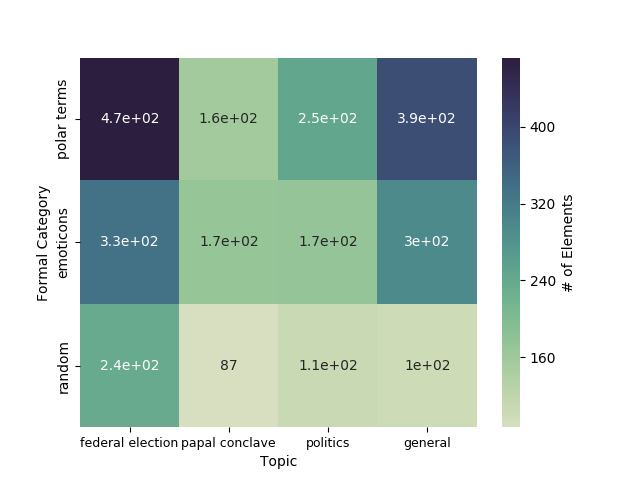
\includegraphics[width=\linewidth]{img/sentiment_stat.png}
  \caption{\texttt{Sentiments}}\label{snt:fig:crp-sent-emo-distr-a}
\end{subfigure}%
\begin{subfigure}{.5\textwidth}
  \centering
  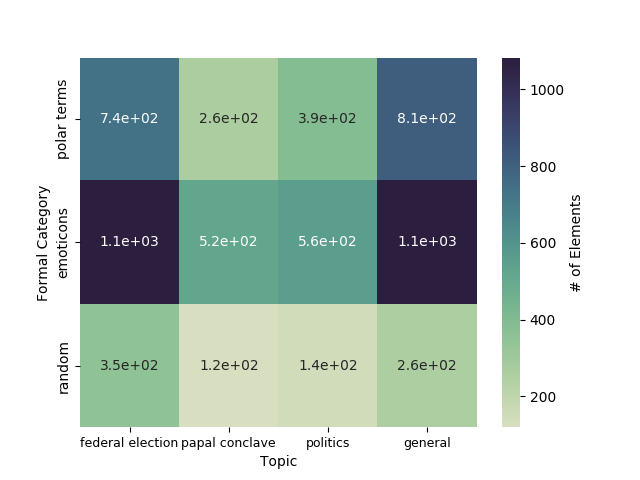
\includegraphics[width=\linewidth]{img/emo-expression_stat.png}
  \caption{\texttt{Polar Terms}}\label{snt:fig:crp-sent-emo-distr-b}
\end{subfigure}
}
\caption{Distribution of sentiments and polar terms across topics and
  formal groups}\label{snt:fig:crp-sent-emo-distr}
\end{figure*}

\begin{figure*}[htbp!]
{
\centering
\begin{subfigure}{.5\textwidth}
  \centering
  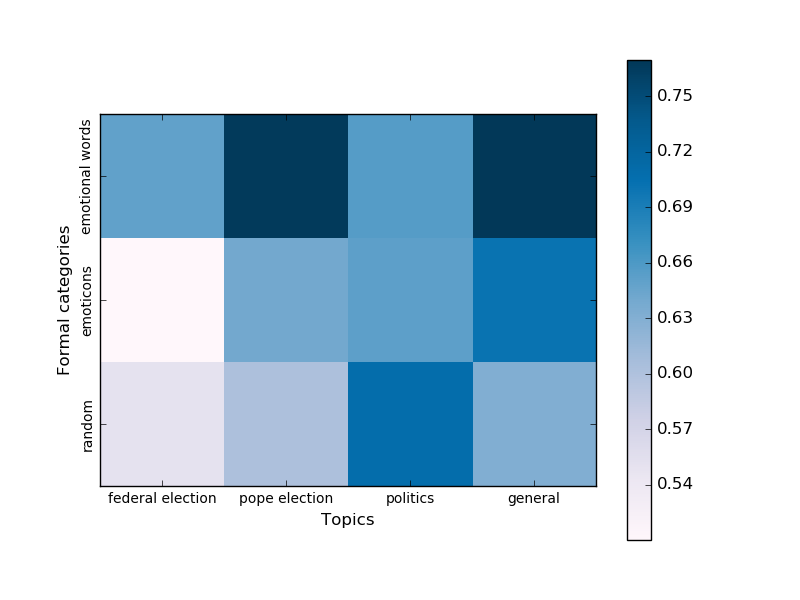
\includegraphics[width=\linewidth]{img/sentiment_agreement.png}
  \caption{\texttt{Sentiments}}
\end{subfigure}%
\begin{subfigure}{.5\textwidth}
  \centering
  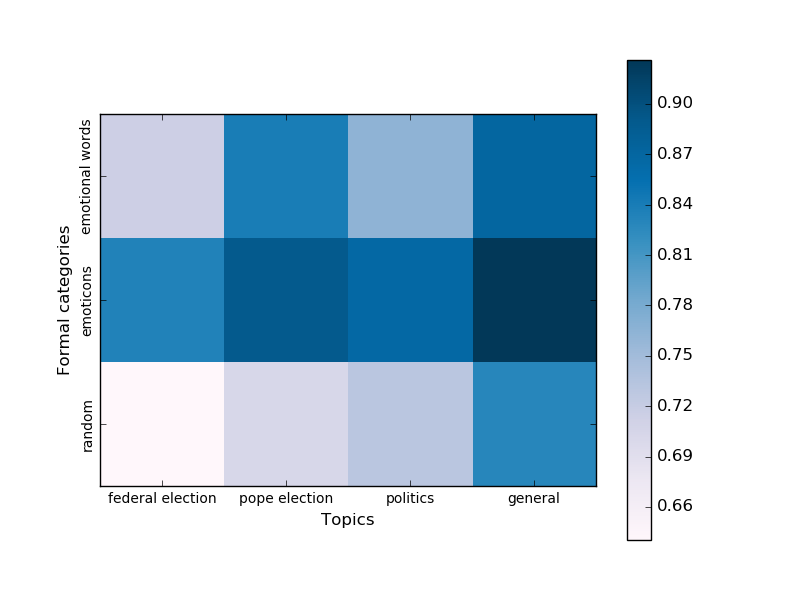
\includegraphics[width=\linewidth]{img/emo-expression_agreement.png}
  \caption{\texttt{Polar Terms}}
\end{subfigure}
}
\caption{Inter-annotator agreement on sentiments and polar terms
  across topics and formal groups}\label{snt:fig:crp-sent-emo-agr}
\end{figure*}

As we can see from the plots, topics and form clearly affect both the
number of opinions and the difficulty of their interpretation.
According to Figure~\ref{snt:fig:crp-sent-emo-distr}, the greatest
number of \markable{sentiment}s occur in tweets pertaining to the
federal elections and in messages representing casual everyday
conversations.  A similar tendency is observed for \markable{polar
  term}s, but in this case, the form of the microblogs seems to have
more impact on the elements' distribution than their topics.

%% Moreover, a higher number of opinionated terms might not necessarily
%% lead to a higher number of targeted sentiments.  We can recognize that
%% from the fact that, even though the biggest number of subjective
%% opinions show up in the first row of
%% Plot~\ref{snt:fig:crp-sent-emo-distr-a} (\ie{} in tweets with terms
%% from the SentiWS lexicon), most of the polar terms appear in row two
%% of Plot~\ref{snt:fig:crp-sent-emo-distr-b} (\ie{} in microblogs
%% containing smileys).

Regarding the inter-annotator agreement, we can see that
\markable{sentiment}s and \markable{polar term}s are most reliably
annotated in messages from the German Twitter Snapshot.  Moreover, the
former elements are apparently easiest to annotate in tweets that were
preselected using a sentiment lexicon, whereas \markable{polar term}s
are easiest to analyze in microblogs that contain emoticons.
%% Somewhat surprisingly, the emoticon group has the lowest IAA scores
%% for \markable{sentiment}s, which means that although our annotators
%% could easily recognize facial expressions as polar items, they had
%% difficulties with determining whether these expressions evaluated
%% something particular in the microblog or reflected the general mood of
%% the author.

To confirm the correlation between the topics and formal groups on the
one hand and the number and reliability of \markable{sentiment}s and
\markable{polar term}s on the other hand, we computed the correlation
coefficients ($\rho$) of these factors.
\begin{table}[thb!]
  \begin{center}
    \bgroup \setlength\tabcolsep{0.47\tabcolsep}\scriptsize
    \begin{tabular}{p{0.2\columnwidth}%
          *{4}{>{\centering\arraybackslash}p{0.185\columnwidth}}} % next five columns
      \toprule

      \multirow{3}{0.2\columnwidth}{\centering\bfseries Selection Criteria} & %
      \multicolumn{4}{c}{\bfseries Correlation Coefficients}\\\cmidrule(lr){2-3}\cmidrule(lr){4-5}

      & \multicolumn{2}{c}{\bfseries Sentiment}& %
      \multicolumn{2}{c}{\bfseries Polar Term}\\\cmidrule(lr){2-2}\cmidrule(lr){3-3}%
      \cmidrule(lr){4-4}\cmidrule(lr){5-5}

      & \# of elements & agreement & \# of elements & agreement\\\midrule

      \multicolumn{5}{c}{\cellcolor{cellcolor}Topical Groups}\\
      Federal Elections & \textbf{0.312} & 0.169 & 0.356 & 0.289\\
      Papal Conclave & 0.149 & 0.124 & 0.182 & 0.264\\
      Political Discussions & 0.195 & 0.148 & 0.218 & 0.244\\
      General Conversations & 0.183 & \textbf{0.19} & \textbf{0.372} & \textbf{0.452}\\
      \multicolumn{5}{c}{\cellcolor{cellcolor}Formal Categories}\\
      Polar Terms & \textbf{0.445} & \textbf{0.352} & 0.38 & 0.301\\
      Emoticons & 0.127 & 0.096 & \textbf{0.47} & \textbf{0.615}\\
      Random & 0.216 & 0.134 & 0.143 & 0.138\\
      \bottomrule
    \end{tabular}
    \egroup
    \caption[Correlation coefficients of topics and selection criteria
      with the number and agreement of sentiments and polar
      terms]{Correlation coefficients of topics and formal selection
      criteria with the number and agreement scores of sentiments and
      polar terms}
    \label{sent:tbl:corr-coeff}
  \end{center}
\end{table}

As we can see from the results in Table~\ref{sent:tbl:corr-coeff},
both criteria (topics and form) have a positive correlation with the
number of annotated elements and their reliability.  The highest
$\rho$-score for \markable{sentiment}s is achieved by the tweets
describing federal elections and messages containing polar terms,
where it amounts to 0.312 and 0.445 respectively.  A slightly
different situation is observed for \markable{polar term}s: the
highest scores for this element both in terms of the number of
annotated items and their reliability are achieved by casual everyday
conversations and tweets that contain emoticons.

%% In general, we can say that, to a greater or lesser extent, virtually
%% every annotation aspect of the resulting corpus except for the
%% sentiment agreement is correlated with the topic or form of the tweets
%% being labeled.  Regarding the uncorrelatednes of the sentiment
%% reliability scores, we hypothesize that the mere task of recognizing
%% subjective opinions in microblogs was so challenging to the human
%% experts (which was also confirmed by our initial annotation
%% experiments) that the difficulties with interpreting the guidelines
%% and applying their instructions to concrete cases have played a much
%% more crucial role and posed much bigger problems to the coders than
%% the particular specifics of topical and formal groups.

%% Based on these statistics, we can already say that the agreement
%% scores achieved in the last stage and the rest of the statistics
%% presented in this section suggest that our assistants could eventually
%% agree not only on the boundaries of sentiment elements but also on the
%% text spans of their respective sources and targets as well as
%% pertaining opinionated terms.  Furthermore, the results shown in
%% Table~\ref{tbl:attr-agrmnt} prove that the polarity and intensity
%% attributes of these elements could be reliably analyzed either.
%% Finally, the statistics plots on the distribution of subjective
%% opinions and polar terms show precisely how different sampling
%% criteria have affected the final composition and agreement scores of
%% the final corpus.

%% \section{Related Work}

%% As we already mentioned in the previous section, most of today's
%% resources for sentiment analysis on Twitter have been either created
%% fully automatically or obtained in a semi-supervised way.  In this
%% category also fall the popular datasets of \citet{Go:09},
%% \citet{Barbosa:10} as well as \citet{Pak:10}, whose message-polarity
%% labels were obtained either based on the emoticons contained in the
%% downloaded messages or taking the majority vote of third-party opinion
%% mining solutions.  Even though these corpora represent valuable
%% sources for developing new classifiers, the possibility of using these
%% data for training is only due to the large size of the collections
%% rather than the quality of their annotations.  Moreover, the
%% coarse-grained nature of the annotation schemes and the inherent
%% noisiness of the labels prevents the researchers from properly
%% analyzing linguistic phenomena in these collections.

%% A notable exception to these works constitutes the SemEval dataset of
%% \citet{Nakov:13}---a set of 15,000 microblogs which were manually
%% analyzed by human experts on the Amazon Mechanical Turk platform.
%% Even though this corpus is one of the biggest manually labeled tweet
%% collections to date, its data still have some potential drawbacks:
%% First of all, all messages included in this tweebank were prefiltered
%% through the SentiWordNet lexicon~\cite{Esuli:06b}, leaving out tweets
%% which did not contain any terms from this resource.  As we showed in
%% the evaluation part of this section, introducing such bias in the
%% sampled data might significantly affect the resulting distribution,
%% omitting many relevant phenomena of interest.  Furthermore, the
%% annotations of this dataset only provide information about the
%% polarity of single lexical items or complete microblogs, losing
%% valuable details about the targets, holders of opinions, and
%% compositionality effects of modifying elements.

%% This scarceness of suitable resources becomes even more aggravated
%% when speaking about Twitter corpora for non-English languages.  A few
%% attempts at creating opinion datasets for microblogs that we are aware
%% of are the sentiment subset of the TWITA corpus \cite{Basile:13} and
%% the Senti-TUT corpus of \citet{Bosco:13} created for Italian, as well
%% as the TASS shared task data \cite{Villena-Roman:13} developed for
%% Spanish.

%% The TWITA collection was used to create a smaller subset of 2,000
%% tweets, which were subsequently manually labeled with their
%% message-level polarities by three human coders.  The Senti-TUT
%% tweebank comprises 3,288 microblogs pertaining to the election of
%% Mario Monti and 1,159 messages obtained from the Twitter section of
%% the popular Italian web portal \url{http://www.spinoza.it}, which were
%% labeled by five annotators with the message-level polarity classes:
%% positive, negative, ironic, mixed, or none.  A different set of
%% sentiment valences (viz., strong negative, negative, neutral,
%% positive, and strong positive) was used for 70,000 messages of the
%% Spanish TASS corpus.

%% To the best of our knowledge, the only sentiment corpus for German
%% Twitter that existed at the time of creating our dataset was the
%% collection of 100,000~messages pertaining the German federal elections
%% 2009 gathered by \citet{Tumasjan:10}.  These tweets were automatically
%% translated into English and annotated with 12 psychological categories
%% (future orientation, past orientation, positive emotions, negative
%% emotions, sadness, anxiety, anger, etc.) using the LIWC program
%% \cite[Linguistic Inquiry and Word Count;][]{Pannebaker:07}.

%% In this regard, our presented corpus makes a valuable contribution to
%% the ecosystem of sentiment analysis data, not only filling the gap of
%% missing manual Twitter corpora with rich annotation schemes but also
%% providing a unique resource for developing new opinion mining systems
%% for German.  %% A detailed inter-annotator agreement study proesented
%% %% in this section proves that our experts could reliably annotate the
%% %% sentiment phenomena in question.  Furthermore, a detailed breakdown
%% %% of different topical and formal tweet categories unequivocally
%% %% shows which groups are more likely to contain evaluative subjective
%% %% judgements and which of these judgements might be more difficult to
%% %% agree on than the others.

\section{Summary and Conclusions}

Now that we have reached the end of the second chapter, we would like
to remind the reader that in this part of the thesis we have presented
a corpus of 7,992 German microblogs that had been manually annotated
by two human experts with sentiments, targets, sources, polar terms,
and their modifying elements.

To collect the initial data for this corpus, we were tracking tweets
about German federal elections, papal conclave, discussions of general
political topics, and casual everyday conversations between spring and
autumn 2013.  Afterwards, we grouped these messages into three classes
(tweets containing polar terms, microblogs that had exclamation marks
or emoticons, and the rest of the messages) and randomly sampled 666
posts from each of these classes for each topic.

%% A rich annotation scheme, which we devised for our dataset, included
%% \markable{sentiment}s, \markable{target}s, \markable{opinion}s,
%% \markable{polar term}s, their \markable{intensifier}s,
%% \markable{diminisher}s, and \markable{negation}s.  With all these
%% elements, we associated extensive sets of attributes, such as
%% \attribute{polarity}, \attribute{intensity}, \attribute{sarcasm},
%% which also had to be specified by the experts during the annotation.

The annotation process was performed in three steps: first, the
annotators labeled one half of the data after minimal training; then,
we automatically highlighted their divergent analyses and asked them
to resolve these differences; finally, our assistants continued with
the analysis of remaining files.

To estimate the inter-rater reliability, we introduced two modified
versions of the established $\kappa$-metric---binary and proportional
kappa---which differ in the way how they treat overlapping annotations
and partial matches.  Using these measures, we estimated the
inter-annotator agreement of our experts at different stages of their
work.  This study showed that, initially, our assistants could hardly
agree on the mere notion of targeted opinions, but their disagreements
could be resolved with the help of the adjudication procedure that we
applied in step two.  Despite a small drop of the IAA scores in the
final stage, all $\kappa$-values still remained at the level of at
least moderate reliability.

Finally, we demonstrated that our initial selection criteria had a
strong impact on the number and agreement of annotated sentiments and
polar terms, with tweets about federal elections and messages without
prefiltered topics being the most prolific sources of these elements.

That way, we not only contributed to the inventory of available
sentiment and social-media resources for German but also provided new
insights into different sampling methods that could be used to create
an opinion dataset and described the consequences of applying these
methods in practice.  A detailed inter-annotator agreement study
showed precisely which topics yield most subjective opinions
(elections and casual conversations) and which groups of messages are
especially difficult to annotate (tweets containing emoticons and
microblogs without polar terms or emoticons).  In the next step, we
are going to check whether our dataset can also serve as a basis for
building and evaluating automatic opinion mining applications.
